% This example is meant to be compiled with lualatex or xelatex
% The theme itself also supports pdflatex
\PassOptionsToPackage{unicode}{hyperref}
\documentclass[aspectratio=1610, 9pt]{beamer}

% Load packages you need here
\usepackage[american]{babel}

\usepackage[autostyle]{csquotes}


\usepackage{amsmath}
\usepackage{amssymb}
\usepackage{mathtools}
\usepackage{xfrac}

\usepackage{tikz}
\usetikzlibrary{arrows.meta}
\usepackage[
  separate-uncertainty=true,
  per-mode=symbol-or-fraction,
]{siunitx}

% nice tables
\usepackage{tabularray}

% colors
\usepackage{xcolor}

\usepackage{hyperref}
\usepackage{bookmark}

% load the theme after all packages

\usetheme[dark]{tudo}

% Put settings here, like
\unimathsetup{
  math-style=ISO,
  bold-style=ISO,
  nabla=upright,
  partial=upright,
  mathrm=sym,
}

\title{ctapipe -- Prototype Open Event Reconstruction Pipeline for the Cherenkov Telescope Array}
\author[M.~Linhoff]{\emph{Maximilian Linhoff}, Lukas Nickel, Noah Biederbeck for the CTA Consortium and Observatory}
\institute[TU Dortmund]{Astroparticle Physics}
\titlegraphic{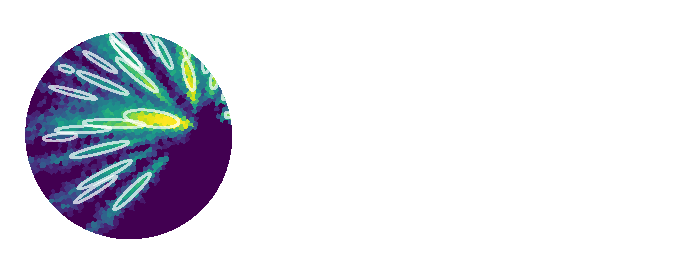
\includegraphics[height=0.4\textheight]{ctapipe-logo-dark.pdf}}


\begin{document}

\maketitle

\begin{frame}{CTA}
\end{frame}

\begin{frame}{ctapipe}
\end{frame}

\begin{frame}
  \begin{tikzpicture}
  \tikzset{datalevel/.style={thick, circle, draw, inner sep=2pt, minimum size=25pt}}
  \tikzset{analysis-step/.style={align=center, font=\footnotesize}}
  \tikzset{step-arrow/.style={-{Triangle Cap}, line width=5pt, shorten >= 5pt, shorten <= 5pt}}

    % raw data plot
    \node[] (R0Graph)   at (0.0, 0) {\includegraphics[height=1.75cm]{build/r0.pdf}};
    \node[] (R1Graph)   at (2.5, 0) {\includegraphics[height=1.75cm]{build/r1.pdf}};
    \node[] (DL0Graph)  at (5.0, 0) {\includegraphics[height=1.75cm]{build/dl0.pdf}};

    \node[] (DL1ImageGraph)   at (10.0, 0.0) {\includegraphics[height=2.5cm]{build/dl1a.pdf}};
    \node[] (DL1CleanGraph) at (10.0, -5) {\includegraphics[height=2.5cm]{build/dl1a_clean.pdf}};

    % Param table
    \node [font=\scriptsize] (DL1bTable) at (1.5, -6) {
      \SetTblrInner{rowsep=0pt, colsep=2pt}
      \begin{tblr}{
          colspec={rrrrcr},
          row{1}={font=\bfseries},
      }
        event &  hillas\_intensity & hillas\_width  & hillas\_length  & $\cdots$ & concentration\_cog \\
          0 &  1253.1    &  0.15  &   0.52  & $\cdots$ & 0.35 \\
          2 &   321.3    &  0.05  &   0.12  & $\cdots$ & 0.42 \\
          5 &   512.7    &  0.08  &   0.19  & $\cdots$ & 0.45 \\
      \end{tblr}
    };

    % Reconstruction table
    \node[font=\scriptsize] (DL2Table) at (1, -3.5) {
        \SetTblrInner{rowsep=0pt, colsep=2pt}
        \begin{tblr}{
            colspec={rrrrrr},
            row{1}={font=\bfseries},
        }
        event & energy & gammaness &    ra &    dec &        time \\
              &        &           &   deg &    deg &        mjd  \\
            0 &   1500 &      0.82 &  83.6 &   22.1 & 59024.63123 \\
            2 &    400 &      0.73 &  83.5 &   21.9 & 59024.64183 \\
            5 &    680 &      0.92 &  83.7 &   22.0 & 59024.67093 \\
        \end{tblr}
    };

    \node [datalevel, color=gray, anchor=north]    (R0)   at (R0Graph.south)   {R0};
    \node [datalevel, color=gray, anchor=north]    (R1)   at (R1Graph.south)   {R1};
    \node [datalevel, anchor=north]                (DL0)  at (DL0Graph.south) {DL0};
    \node [datalevel, anchor=east, xshift=1.3cm, yshift=-0.1cm] (DL1Image) at (DL1ImageGraph.south west) {DL1a};
    \node [datalevel, anchor=east, xshift=0.7cm, yshift=-0.1cm] (DL1Clean) at (DL1CleanGraph.north west) {DL1a};
    \node [datalevel, anchor=west] (DL1b) at (DL1bTable.east) {DL1b};
    \node [datalevel, anchor=west] (DL2)  at (DL2Table.east) {DL2};

    \draw[step-arrow, color=gray] (R0.east) -- (R1.west)  node [analysis-step, midway, below, text width=2cm] {Low-Level\\Calibration};
    \draw[step-arrow, color=gray] (R1.east) -- (DL0.west)  node [analysis-step, midway, below, text width=2cm] {Data Volume\\ Reduction};
    \draw[step-arrow] (DL0.east) -- (DL1Image.west)  node [analysis-step, midway, below, yshift=-0.15cm] {Pulse Extraction};
    \draw[step-arrow] (DL1Image.south east) to[out=315, in=45]  node [analysis-step, midway, right, xshift=0.2cm] {Image Cleaning} (DL1Clean.north east); 
    \draw[step-arrow] (DL1Clean.south) to[bend left] node [analysis-step, midway, above, xshift=-0.7cm, yshift=0.3cm] {Parametrization} (DL1b.east);
    \draw[step-arrow] (DL1b.110) -- (DL2.south east)  node [analysis-step, midway, left, yshift=-0.2cm] {Reconstruction};

\end{tikzpicture}

\end{frame}

\end{document}
